\begin{figure}[H]
\centering
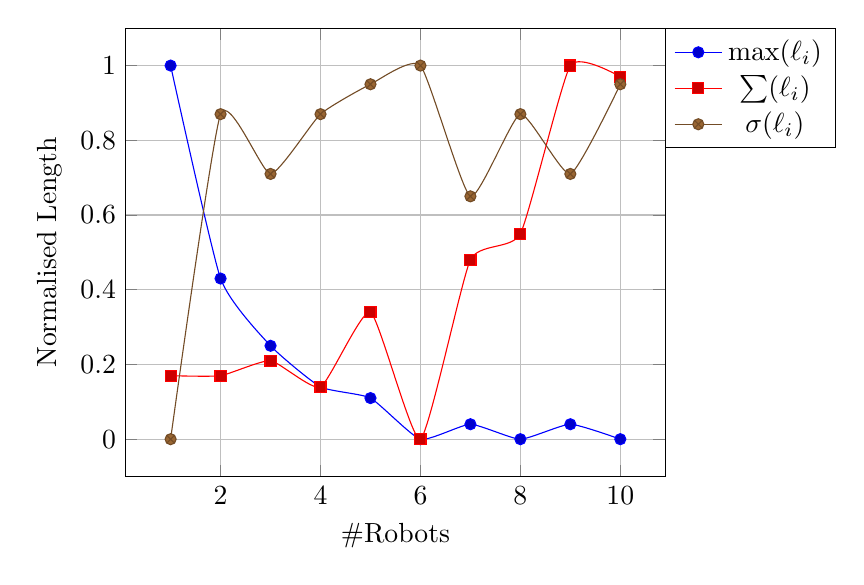
\begin{tikzpicture}
	\begin{axis}[
%		height=9cm,
%		width=9cm,
		grid=major,
                legend style = {at={(1,1)}, anchor=north west},
		xlabel=\#Robots,
		ylabel=Normalised Length,
		smooth,
		tension=0.3
	]

	\addplot coordinates {
(1, 1.00)
(2, 0.43)
(3, 0.25)
(4, 0.14)
(5, 0.11)
(6, 0.00)
(7, 0.04)
(8, 0.00)
(9, 0.04)
(10, 0.00)
	};
	\addlegendentry{$\max(\ell_i)$}

	\addplot coordinates {
(1, 0.17)
(2, 0.17)
(3, 0.21)
(4, 0.14)
(5, 0.34)
(6, 0.00)
(7, 0.48)
(8, 0.55)
(9, 1.00)
(10, 0.97)
	};
	\addlegendentry{$\sum(\ell_i)$}

	\addplot coordinates {
(1, 0.00)
(2, 0.87)
(3, 0.71)
(4, 0.87)
(5, 0.95)
(6, 1.00)
(7, 0.65)
(8, 0.87)
(9, 0.71)
(10, 0.95)
	};
	\addlegendentry{$\sigma(\ell_i)$}
	\end{axis}
\end{tikzpicture}
\caption[Perform. indexes increasing the \#robots, 5x5 grid using NC]{Performance indexes increasing the num. of robots, 5x5 grid using NC}
\end{figure}